%
% karte.tex
%
% (c) 2024 Prof Dr Andreas Müller
%
\begin{figure}
\centering
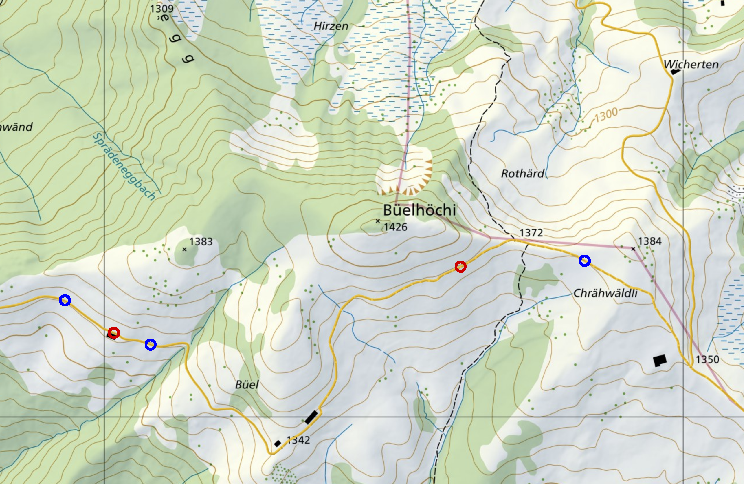
\includegraphics{chapters/010-fuvar/images/karteextremum.pdf}
\caption{Lokale Maxima ({\color{darkred}rote} Kreise) und Minima
({\color{blue}blaue} Kreise) der Höhe entlang eines Wanderwegs
({\color{gelb}gelb}) sind Lösungen eines Extremalproblems.
Die Nebenbedingung ist der Wanderweg, der einschränkt, wo der Wanderer
sich bewegen kann.
Die zu optimierenden Grösse $f(x,y)$ ist die Höhe.
Extreme treten an stellen auf, wo die Höhenlinien, die Niveaulinien 
von $f$ und der Wanderweg parallel verlaufen.
\label{buch:fuvar:nebenbedingung:fig:karte}}
\end{figure}
